\section{Robot and Environment}
To test the controller, a robot developed by Topy was at disposal. This is a commercially available robot with its own controller. In order to replace this controller with the haptic feedback controller from this project, it was necessary to write a properly working environment. The topy robot is communicating via a wireless serial link. It has a prespecified communication message that consists in $70$ bytes for sending from the robot to the PC and $44$ bytes for the message to receive. These messages include the bytes reserved for proper starting and ending as well as the checksum. The full documentation of the messages and robot usage can be seen in the Topy manual (Japanese only). \\
It was thus necessary to write an application that reads out the position of the two joysticks and construct a message including these joystick values as speed reference for the robot. Then the message has to be sent over the wireless serial link to the robot and the answer has to be received. The important sensor readings (inclination, current in the crawlers, passed time and battery level) have to be read out and a feedback according to the chosen feedback law has to be sent to the motors.\\
For this purpose, the programming language processing \cite{Fry2018} has been used to create a graphical user interface and to establish the serial connection. For low-level motor control purposes an Arduino Uno has been used. The parameters that can be set for testing purposes can be seen in table \ref{tab:programming_params}.
	
\begin{figure}[h!]
	\centering
	\begin{tabular}{|l|c|l|}
			
		\hline
		Setting & Value & Units \\ \hline \hline
		Baud rate for robot serial link & $250000$ & [bps]\\ \hline
		Baud rate for Arduino serial link & $250000$ & [bps] \\ \hline
		Update rate of the processing GUI & $5$ & [Hz] \\ \hline
		Update rate of the Arduino motor controller & $1000$ & [Hz] \\ \hline
		Max voltage for motor & $20$ & [V] \\ \hline
		%TODO write this? Feedback resolution & 5 out of 255 & [-] \\ \hline
		PWM frequency & $31372.55$ & [Hz]  \\ \hline
		Proportional motor gain & $47.6$  & [V/mm] \\ \hline
		Integral motor gain & $0.124$  & [V/mm/s]\\ \hline
		Derivative motor gain & $247$  & [Vs/mm]\\ \hline
		Feedback filter cut-off frequency  & $160$ & [Hz] \\ \hline %TODO calculate cut off frequency
		Left photoreceptor MIN value & $640$ & [-] \\ \hline
		Left photoreceptor MAX value & $840$ & [-] \\ \hline
		Right photoreceptor MIN value & $700$ & [-] \\ \hline
		Right photoreceptor MAX value & $880$ & [-] \\ \hline		
	\end{tabular}
	\caption{Software parameters.}
	\label{tab:programming_params}
\end{figure}
	
	

\subsection{GUI in Processing}
The graphical user interface shows the current feedback method as well as the magnitude. It also indicates which driving direction (forward, backward or halt) is sent to the robot. Since there is no control of the battery charge on-board, the robot sends battery information in its message to the PC. The processing program reads out the charge of the battery and warns the user if it is too low. It stops the program, if the battery state is critical. The feedback method can be changed by a mouse-click anywhere in the window. The GUI can be seen in figure \ref{fig:processing_gui}.
	 
\begin{figure}[h!]
	\centering
	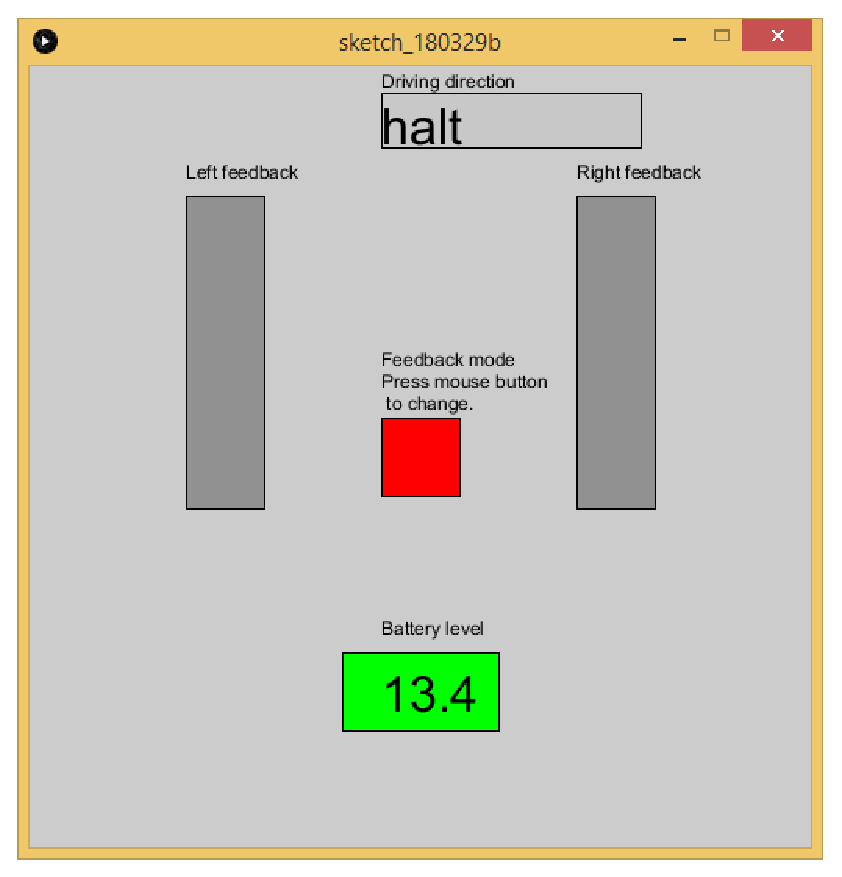
\includegraphics[width=0.4\linewidth]{Figs/processing_gui}
	\caption{Graphical user interface written in processing.}	\label{fig:processing_gui}
\end{figure}

This application handles the messages sent to and from the robot. The communication between the GUI and the Arduino is over the serial cable with a fixed baud rate (see table \ref{tab:programming_params}). The same baud rate has been used for the communication between the GUI and the real robot. The latter communication frequency is of $5$Hz, which has been suggested by the Topy user manual. 
	
\subsection{Control Scheme}
The control scheme is based on a simple proportional controller. The scheme can be seen in figure \ref{fig:control_scheme}. In the test setup (see section \ref{sec:ps_testing}) the reference signal $dist_{ref}$ is given by the sinusoidal function generator. This reference signal is directly treated as desired feedback. In the operational mode, this corresponds to the target output force, also called the haptic feedback force that should be felt by the user. Ideally, this shall be a function of orientation (roll and pitch) as well as the current in the two crawlers.
	
\subsection{Electrical low-pass Filter}
Before the PWM signal from the Arduino is sent to the amplifiers, where it is amplified to control the motors, it has been filtered with a simple RC low-pass filter. The resistor has a value of $3.9$ k$\Omega$ and the capacitor of $0.1$ $\mu$F. This smooths out the PWM signal and has been implemented in order to avoid that the amplifier tries to follow the Arduino signal with unnecessary precision, eventually causing too much heat. The cut-off frequency is therefore $ 204$Hz.




\newpage